\chapter{실험}\label{chap:experiments}

이 장에서는 세 가지 실험을 다룬다. \ref{sec:exp-latency}절에서는 two-line 모델을 실험 장치의 읽기 비용에 적합하고, \ref{sec:exp-model}절에서는 이 비용 모델 아래에서 선택 방법들을 최적해와 비교하며, \ref{sec:exp-real}절에서는 행을 선택하는 시간과 SSD에서 읽는 시간을 직접 측정한다. 모든 실험은 표~\ref{tab:environment}의 노트북 한 대에서 수행하였다.

\begin{table}[htbp]
    \centering
    \caption{실험 장치}
    \label{tab:environment}
    \begin{tabular}{ll}
        \toprule
        항목 & 사양 \\
        \midrule
        기기 & Lenovo IdeaPad Pro 5 16AHP9 \\
        CPU & AMD Ryzen 7 8845HS (8코어 16스레드) \\
        GPU & NVIDIA GeForce RTX 3050 Laptop (6 GB) \\
        SSD & WD\_BLACK SN850X 1 TB (NVMe, PCIe 4.0 x4) \\
        파일 시스템 & btrfs, I/O 스케줄러 \texttt{none} \\
        운영체제 & Fedora Linux 44 (kernel 7.2.10) \\
        \bottomrule
    \end{tabular}
\end{table}

\section{Chunk 크기에 따른 SSD 읽기 비용}\label{sec:exp-latency}

이번 실험에서는 \ref{sec:two-line}절에서 도입한 two-line 모델이 실험 장치의 읽기 비용을 얼마나 잘 근사하는지 살펴보았다. Chunk 크기별 읽기 비용에 모델을 적합하고, 별도의 반복 측정값으로 오차를 평가하여 \ref{sec:exp-model}절의 알고리즘 비교에 사용할 비용 함수를 정한다.

\subsection{측정 설정}\label{sec:exp-latency-setup}

노트북의 SSD에 저장한 128 MiB 파일을 대상으로, 6개 스레드와 O\_DIRECT를 사용하여 읽기 비용을 측정하였다. 조사한 chunk 크기는 다음 두 구간의 432개이다.

\begin{itemize}
\item 1--320 KiB: 1 KiB 간격
\item 324--768 KiB: 4 KiB 간격
\end{itemize}

한 크기의 처리량은 \ref{sec:neuron-chunking}절에서 설명한 비용 측정 방식에 따라 다음 순서로 추정하였다.

\begin{enumerate}
\item 같은 크기의 chunk 사이에 32 KiB를 비워 두고, chunk 수를 늘려 가며 읽는다.
\item 각 읽기 조건에서 3회 warmup 후 10회 측정하고, 그 시간의 중앙값을 사용한다.
\item 처리량의 변화가 작아지는 구간을 찾아 대표 처리량을 추정한다.
\end{enumerate}

전체 크기 범위에 대한 측정은 7회 반복하였다. 각 반복에서는 크기를 방문하는 순서를 무작위로 섞어, 항상 같은 순서로 측정할 때 발생할 수 있는 영향을 줄였다.

요청 크기를 $z$ KiB, 반복 $t$에서 추정한 처리량을 $\widehat\beta_t(z)$ MiB/s라 하자. 이를 chunk당 읽기 비용으로 환산하면
\[
T_t(z)=\frac{1000z}{1024\widehat\beta_t(z)}
\qquad \mathrm{ms/chunk}
\]
이다. 이후 모델에 적합하는 값은 이처럼 배치 처리량으로 환산한 chunk당 비용이다. 처리량 계산에는 O\_DIRECT 정렬을 위한 padding을 제외한 논리적 요청 크기를 사용하였다.

\subsection{모델의 적합과 평가}\label{sec:exp-latency-fit}

7회 반복 중 앞의 4회를 \textbf{train 자료}, 나머지 3회를 \textbf{test 자료}라 부른다. 모델의 계수와 전환점은 모두 train 자료만으로 결정하고, 오차는 적합에 쓰지 않은 test 자료로 평가하였다. 각 요청 크기에서 train 자료의 중앙값을 $T_{\mathrm{train}}(z)$, test 자료의 중앙값을 $T_{\mathrm{test}}(z)$라 하자.

모델 적합에는 행 수 대신 요청 크기 $z$를 사용한다. \ref{sec:two-line}절의 $\alpha,\lambda,\ell_0$에 대응하는 KiB 단위 계수와 전환점을 각각 $\alpha_z,\lambda_z,z_0$라 하자. 가중치 한 행의 크기가 $w$ KiB이면 $z=w\ell$이므로, 행 단위 모델과는 다음 관계를 갖는다.
\[
\alpha=w\alpha_z,
\qquad
\lambda=w\lambda_z,
\qquad
\ell_0=\frac{z_0}{w}.
\]
적합한 모델은 다음 세 가지이다.

\begin{itemize}
\item \textbf{Two-line}: \ref{sec:two-line}절의 모델이다. 계수 제약을 유지하면서, 측정한 각 크기를 전환점 후보로 두고 비음수 최소제곱법으로 계수를 적합하였다. 그중 train RMSE가 가장 작은 전환점을 선택하였다.
\item \textbf{Hinge}: 연속된 두 직선으로 구성된 비교 모델이다. 큰 요청에서 비용이 요청 크기에 정비례해야 한다는 제약을 두지 않는다. 전환점은 two-line과 같이 train RMSE로 선택하였다.
\item \textbf{Affine}: 하나의 직선으로 구성된 비교 모델이다.
\end{itemize}

두 비교 모델의 식은 다음과 같다.
\[
\begin{aligned}
T_{\mathrm H}(z)&=a_{\mathrm H}+b_{\mathrm H}z+c_{\mathrm H}(z-z_{\mathrm H})_+,\\
T_{\mathrm A}(z)&=a_{\mathrm A}+b_{\mathrm A}z.
\end{aligned}
\]
모든 크기에 같은 가중치를 부여하였으므로, 측정 간격이 촘촘한 320 KiB 이하 구간이 더 많은 관측값을 제공한다.

평가에는 두 지표를 사용한다. 적합된 모델의 예측값을 $\widehat T(z)$, 432개 요청 크기의 집합을 $\mathcal Z$라 하면, test 자료에 대한 두 지표는
\[
\mathrm{RMSE}=\sqrt{\frac{1}{|\mathcal Z|}\sum_{z\in\mathcal Z}\bigl(\widehat T(z)-T_{\mathrm{test}}(z)\bigr)^2},
\qquad
\mathrm{MAPE}=\frac{100}{|\mathcal Z|}\sum_{z\in\mathcal Z}\frac{\bigl|\widehat T(z)-T_{\mathrm{test}}(z)\bigr|}{T_{\mathrm{test}}(z)}
\]
이다. \textbf{RMSE}는 비용 예측의 절대적인 오차 크기를, \textbf{MAPE}는 측정 비용 대비 절대 오차의 평균 비율을 나타낸다. Train RMSE는 같은 식에서 $T_{\mathrm{test}}$ 대신 $T_{\mathrm{train}}$을 사용한 값이다.

\subsection{결과와 해석}\label{sec:exp-latency-results}

그림~\ref{fig:throughput}\은 측정한 모든 요청 크기에서의 처리량을 보여준다. 처리량은 작은 요청에서 크기와 함께 빠르게 오르다가 240 KiB 부근에서 포화한다. Train 자료에서 처리량이 가장 높은 측정 크기는 240 KiB였다. 처리량에 3점 이동 중앙값을 적용한 뒤 최고값의 99\%에 처음 도달한 크기는 233 KiB였다.

\begin{figure}[htbp]
    \centering
    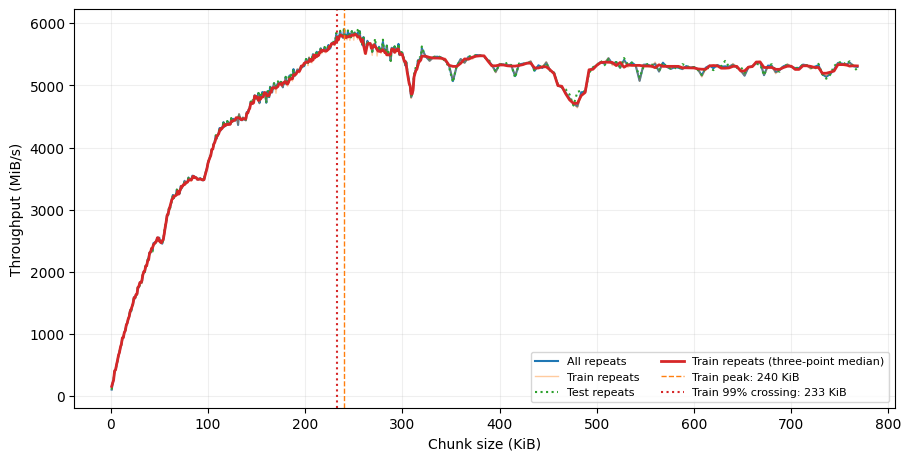
\includegraphics[width=0.8\textwidth]{figures/01/01_throughput.png}
    \caption{전체·train·test 자료의 읽기 비용 중앙값으로 환산한 처리량. 수직선은 train 자료의 최고 처리량 위치와, 3점 이동 중앙값을 적용한 처리량의 99\% 도달 위치를 나타낸다.}
    \label{fig:throughput}
\end{figure}

Two-line 모델의 전환점은 $z_0=208$ KiB로 선택되었다. 이 값은 전체 측정 크기에 대한 train RMSE를 최소화한 결과이며, 위의 두 처리량 지표와는 구분한다. 적합된 모델은 이 전환점에서 꺾이며, $z$를 KiB, 비용을 µs로 두면
\[
T_{\mathrm{2L}}(z)\approx
\begin{cases}
12.22+0.1251\,z, & 0<z<208,\\
0.1838\,z, & z\ge208
\end{cases}
\]
이다. \ref{sec:two-line}절의 기호로는 $\alpha_z\approx0.1838\;\mathrm{\mu s/KiB}$, $\lambda_z\approx0.0588\;\mathrm{\mu s/KiB}$이다.

그림~\ref{fig:model-fit}\는 test 자료의 측정값과 각 모델의 예측 곡선을 비교한다. 표~\ref{tab:fit-errors}에는 전환점을 적합한 two-line 및 hinge 모델과 affine 모델의 오차를 정리하였다.

\begin{figure}[htbp]
    \centering
    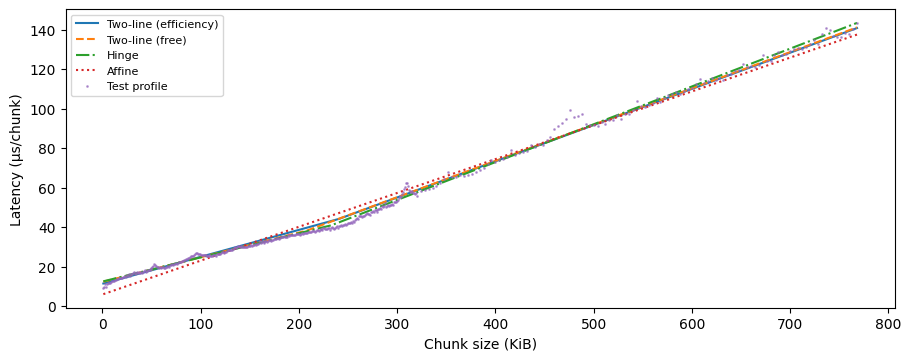
\includegraphics[width=0.8\textwidth]{figures/01/02_model_fit.png}
    \caption{요청 크기별 읽기 비용의 측정값과 모델 예측. Test profile은 test 자료의 중앙값이다. Two-line (free)는 표~\ref{tab:fit-errors}의 Two-line 모델이며, Two-line (efficiency)는 전환점을 최고 처리량 크기인 240 KiB로 고정한 비교 설정이다.}
    \label{fig:model-fit}
\end{figure}

\begin{table}[htbp]
    \centering
    \caption{모델별 전환점과 적합 오차}
    \label{tab:fit-errors}
    \begin{tabular}{lrrrr}
        \toprule
        모델 & 전환점 (KiB) & Train RMSE (µs) & Test RMSE (µs) & Test MAPE (\%) \\
        \midrule
        Two-line & 208 & 2.076 & 2.043 & 3.415 \\
        Hinge & 233 & 1.814 & 1.731 & 2.707 \\
        Affine & --- & 3.887 & 3.909 & 10.467 \\
        \bottomrule
    \end{tabular}
\end{table}

Two-line 모델은 affine 모델보다 작은 test 오차를 보였으며, test RMSE는 2.043 µs, test MAPE는 3.415\%였다. Train RMSE와 test RMSE도 비슷하여, 적합에 사용하지 않은 반복 측정에서도 유사한 근사 정확도를 보였다. 다만 비교 모델 중 test 오차가 가장 작은 것은 hinge 모델이었다.

크기별 오차를 더 자세히 보기 위해, 그림~\ref{fig:residuals}에 예측값에서 test 자료의 측정값을 뺀 잔차를 나타내었다. 예를 들어 약 480 KiB에서는 여러 모델이 실제 읽기 비용을 낮게 예측하며, 이는 그림~\ref{fig:throughput}에서 나타난 처리량 하락과 대응한다.

\begin{figure}[htbp]
    \centering
    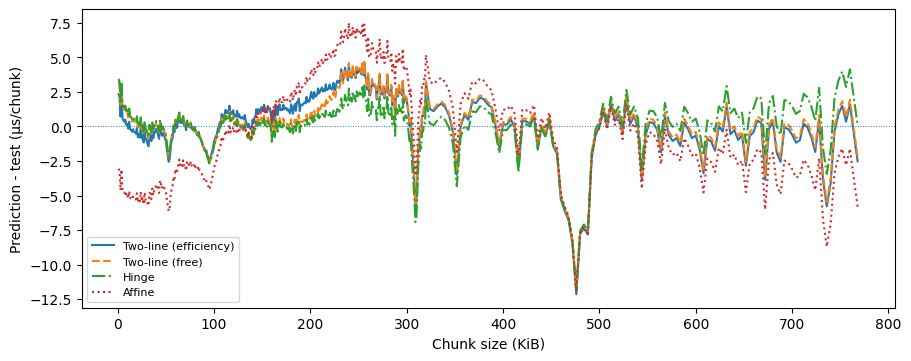
\includegraphics[width=0.8\textwidth]{figures/01/03_residuals.png}
    \caption{요청 크기별 예측 잔차. 양수는 읽기 비용의 과대 예측, 음수는 과소 예측을 의미한다.}
    \label{fig:residuals}
\end{figure}

이처럼 실측 처리량에는 요청 크기에 따른 국소적인 변동이 남아 있다. \ref{sec:two-line}절에서 둔 일정한 포화 처리량은 이러한 변동을 단순화한 근사 조건이며, 이 실험에서는 그에 따른 오차를 평가하였다.

\section{비용 모델에서의 선택 알고리즘 비교}\label{sec:exp-model}

이번 실험에서는 \ref{sec:exp-latency}절에서 적합한 two-line 모델을 사용하여, Global DP, Paper, Tiles, Top-$R$의 보존 중요도와 추정 읽기 비용을 비교하였다. \ref{sec:dp}절의 Global DP를 고정 행 예산에서의 비율 최적해로 두고, 각 선택 방법이 이 기준에 얼마나 가까운지 살펴본다. 이 절의 지연시간은 비용 모델의 추정값이며, 행을 선택하는 계산 시간과 실제 SSD 읽기 시간은 \ref{sec:exp-real}절에서 다룬다.

\subsection{입력 자료와 비용 모델}\label{sec:exp-model-input}

중요도는 실제 언어 모델을 실행하여 얻었다. Qwen2.5-0.5B-Instruct\footnote{\url{https://huggingface.co/Qwen/Qwen2.5-0.5B-Instruct}}에 세 개의 텍스트 입력을 주고, attention과 MLP의 projection에 들어가는 activation을 수집하였다. 채널별 activation 절댓값의 평균을 그 채널의 중요도로 삼았으며, 이 중요도 벡터 하나를 trace라 부른다. 총 504개 trace를 사용하였다.

가중치는 원소당 2바이트이며, 입력 채널별 가중치를 한 행으로 배열했을 때 행 수를 $N$, 행당 원소 수를 $D$라 하자. Projection의 크기 $N\times D$는 다음 네 가지이다.

\begin{itemize}
\item $896\times128$
\item $896\times896$
\item $896\times4864$
\item $4864\times896$
\end{itemize}

모든 방법에 \ref{sec:exp-latency}절에서 적합한 two-line 모델을 적용하였다. 한 행의 크기가 $w$ KiB이면 전환점은 $\ell_0=208/w$행이며, 예를 들어 $896\times896$에서는 $w=1.75$이므로 $\ell_0\approx118.86$이다. 선택된 행들을 최대 연속 구간으로 합친 뒤 각 구간의 비용을 더하여 $L(M)$을 계산하였다.

각 trace에서 요청 행 비율을 $f\in\{0.1,0.2,\ldots,0.9\}$로 바꾸며
\[
R=\max\{1,\lfloor fN\rfloor\}
\]
개의 행을 예산으로 주었다.

\subsection{비교 방법과 평가 지표}\label{sec:exp-model-methods}

비교한 방법은 다음 네 가지이다.

\begin{itemize}
\item \textbf{Global DP}: 정확히 $R$개 행을 선택하면서 $I(M)/L(M)$을 최대화하는 \ref{sec:dp}절의 방법이다. 다른 방법을 평가하는 기준으로 사용한다.
\item \textbf{Top-$R$}: 중요도가 가장 큰 $R$개 행을 선택한다.
\item \textbf{Tiles}: \ref{sec:tiles}절의 방법이다. 타일 길이는 전환점을 올림한 $B=\lceil\ell_0\rceil$을 기본으로 하고, 이보다 길거나 짧은 길이도 함께 시험하였다.
\item \textbf{Paper}: \ref{sec:neuron-chunking}절의 greedy 방법이다. 다른 방법과 같은 two-line 비용을 제공하였다.
\end{itemize}

Global DP, Tiles, Top-$R$은 예산을 모두 채우지만, Paper는 더 적은 행을 선택할 수 있다. 비교에는 각 방법이 실제로 반환한 mask의 중요도와 비용을 사용하였다.

평가에는 두 지표를 사용한다. \textbf{보존 중요도}는 전체 중요도 중 mask가 보존한 비율이다. \textbf{DP 대비 비율}은 같은 trace와 요청 예산에서, 각 방법의 중요도--지연시간 비율을 Global DP의 값으로 나눈 것이다. \ref{sec:guarantee}절과 같이 $q(M)=I(M)/L(M)$이라 쓰고 Global DP의 mask를 $M_{\mathrm{DP}}$라 하면, 두 지표는 차례로
\[
100\cdot\frac{I(M)}{\sum_i v_i},
\qquad
100\cdot\frac{q(M)}{q(M_{\mathrm{DP}})}
\]
이며 단위는 \%이다. 아래의 수치는 모두 trace 간 중앙값이며, DP 대비 비율은 trace마다 먼저 계산한 뒤 중앙값을 구하였다.

\subsection{중요도와 추정 읽기 비용}\label{sec:exp-model-results}

그림~\ref{fig:model-importance}\은 $896\times896$에서 요청 예산을 바꾸었을 때의 결과이다. 각 점은 하나의 trace이며, 같은 예산에서 중요도와 지연시간의 중앙값을 각각 구하여 연결하였다. 점선은 Global DP의 중앙값을 나타낸다.

\begin{figure}[htbp]
    \centering
    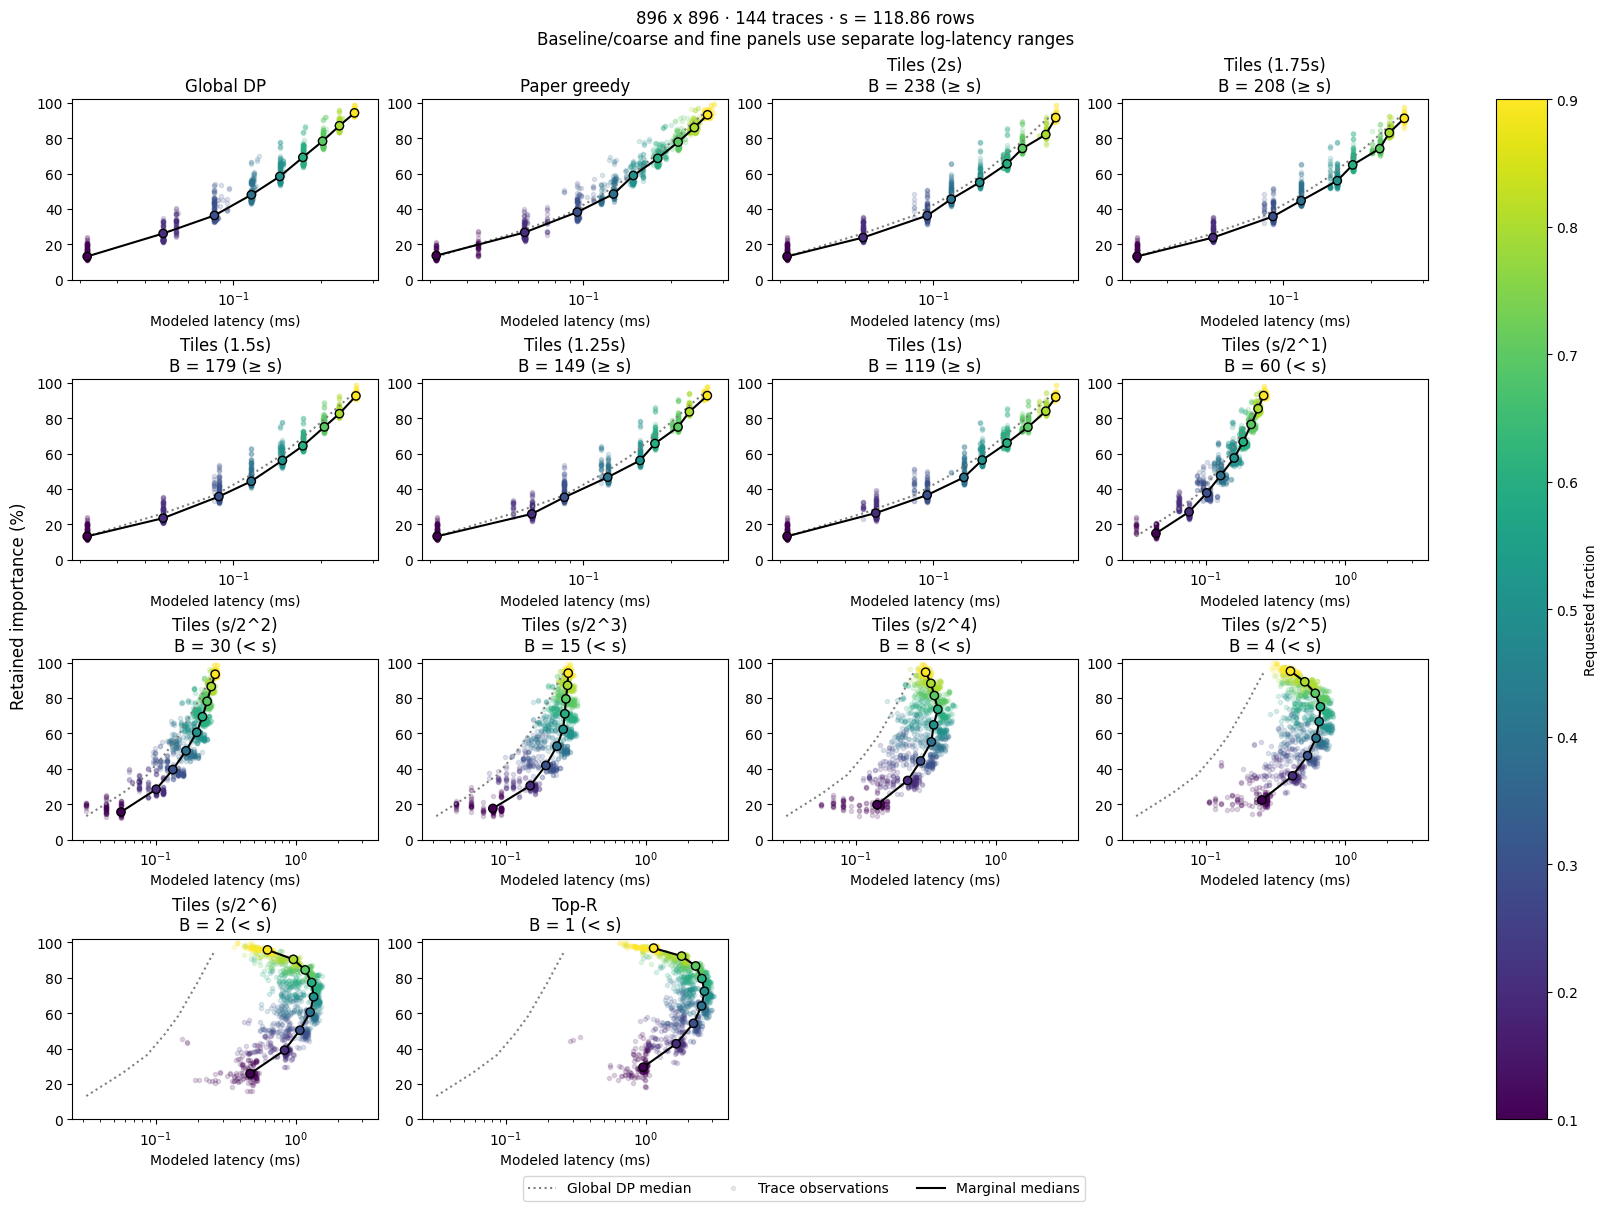
\includegraphics[width=0.85\textwidth]{figures/02/01_importance_latency_896x896.png}
    \caption{요청 행 비율에 따른 보존 중요도와 two-line 추정 읽기 비용. 색은 요청 비율을 나타내며, 그림의 s는 행 단위 전환점이다. Baseline/coarse와 fine 패널은 서로 다른 가로축 범위를 사용하고, 가로축은 로그 척도이다.}
    \label{fig:model-importance}
\end{figure}

요청 비율이 50\%일 때는 $R=448$이다. 이 예산에서 네 방법의 결과를 정리하면 표~\ref{tab:model-50}\와 같다. Tiles는 $B=\lceil\ell_0\rceil=119$인 설정을 사용하였다.

\begin{table}[htbp]
    \centering
    \caption{$896\times896$, 50\% 예산에서의 보존 중요도와 추정 읽기 비용 (trace 간 중앙값)}
    \label{tab:model-50}
    \begin{tabular}{lrrr}
        \toprule
        방법 & 보존 중요도 (\%) & 추정 읽기 비용 (ms) & DP 대비 비율 (\%) \\
        \midrule
        Global DP & 58.44 & 0.1441 & 100.00 \\
        Paper & 58.97 & 0.1483 & 96.82 \\
        Tiles ($B=119$) & 56.32 & 0.1470 & 95.87 \\
        Top-$R$ & 72.48 & 2.6400 & 7.22 \\
        \bottomrule
    \end{tabular}
\end{table}

Top-$R$은 중요도를 가장 많이 보존하지만, 추정 읽기 비용이 다른 세 방법의 열 배를 넘는다. Tiles와 Paper는 Top-$R$보다 중요도를 덜 보존하는 대신 읽기 비용을 Global DP와 거의 같은 수준으로 낮추었고, 두 방법 모두 최적 비율의 96\% 안팎에 도달하였다.

나머지 세 shape에서도 같은 50\% 예산에서 Tiles와 Paper의 DP 대비 비율은 모두 95\%를 넘었고, Top-$R$은 27\%에 미치지 못하였다. Tiles와 Paper를 비교하면, 네 shape 중 세 곳에서 Paper의 비율이 약 1--2\%p 높았다.

% 작성 근거: 기존 노트북의 코드와 저장된 결과를 읽어 작성하였으며 실험은 재실행하지 않았다.
% 입력 수집: ../../results/02/02_01_capture_traces.ipynb
% 비율 최적해: ../../results/02/02_02_global_oracle.ipynb
% 선택 방법과 설정: ../../results/02/02_03_selector_sweep.ipynb
% 그림 fig:model-importance: ../../results/02/02_04_analyze_oracle.ipynb, cells[16].outputs[1].data[image/png]
% PNG는 저장된 출력에서 그대로 추출하였다.
% 표와 본문의 수치: ../../results/02/02_06_report_numbers.ipynb (oracle_reference.csv 및 selector_results.csv에서 계산)
% 보존 중요도 = 100 * importance / importance_total.
% DP 대비 비율 = 100 * (importance / latency) / (DP importance / DP latency).
% DP 결과는 trace_id와 fraction으로 대응시키고, shape·방법·예산별 중앙값을 구하였다.

\section{실제 선택 시간과 SSD 읽기 시간 비교}\label{sec:exp-real}

이번 실험에서는 Paper, Tiles, Top-$R$을 실제로 실행하고, 선택한 행들을 SSD에 저장한 파일에서 읽는 시간을 측정하였다. \ref{sec:exp-model}절의 지연시간은 비용 모델의 추정값이었고, 행을 선택하는 계산에 걸리는 시간은 다루지 않았다. 여기서는 행을 선택하는 시간과 SSD에서 읽는 시간을 직접 측정하여 두 가지를 확인한다. 첫째는 \ref{sec:exp-model}절에서 추정한 방법 간 읽기 비용의 관계가 \textbf{실제 읽기 시간}에서도 나타나는지이고, 둘째는 \textbf{행을 선택하는 계산 시간}을 포함하면 방법 간 차이가 어떻게 달라지는지이다. Global DP는 이번 실측 비교에 포함하지 않았다.

\subsection{측정 설정}\label{sec:exp-real-setup}

\ref{sec:exp-model}절의 중요도 자료에서 shape별로 저장 순서상 균등한 간격의 32개 trace를 골라, 총 128개를 사용하였다. 요청 행 비율은 $f\in\{0.3,0.4,\ldots,1.0\}$으로 바꾸었으며, 행 예산은 \ref{sec:exp-model}절과 같이
\[
R=\max\{1,\lfloor fN\rfloor\}
\]
이다.

읽는 대상은 임의 바이트로 채워 SSD에 저장한 파일이다. 행마다 실제 가중치와 같은 바이트 수를 갖도록 파일의 행을 해석하고, 선택한 행 위치에 해당하는 데이터를 읽었다. 읽기에는 \ref{sec:exp-latency}절과 같이 최대 6개 스레드와 O\_DIRECT를 사용한다. 실제 모델 가중치를 사용한 추론은 이 측정에 포함하지 않는다.

각 trace와 예산에서 3회 warmup 뒤 30회 측정하였다. 매 반복에서 방법의 실행 순서를 무작위로 섞었고, 방법마다 mask를 다시 계산한 뒤 읽기를 수행하였다.

\subsection{측정한 세 가지 시간}\label{sec:exp-real-times}

한 번의 반복에서 표~\ref{tab:real-times}의 세 시간을 따로 기록하였다.

\begin{table}[htbp]
    \centering
    \caption{한 번의 반복에서 기록한 세 가지 시간}
    \label{tab:real-times}
    \begin{tabular}{ll}
        \toprule
        시간 & 측정 범위 \\
        \midrule
        \textbf{선택 시간} & 미리 준비된 중요도에서 읽을 행의 mask를 구성하는 시간 \\
        \textbf{읽기 시간} & Reader가 그 mask의 행들을 읽는 시간 \\
        \textbf{전체 시간} & 선택을 시작한 때부터 읽은 데이터를 반환할 때까지의 시간 \\
        \bottomrule
    \end{tabular}
\end{table}

전체 시간에는 읽기 요청과 버퍼를 준비하는 시간도 들어 있다. 따라서 전체 시간은 선택 시간과 읽기 시간의 합보다 조금 크다.

trace·예산·방법의 조합 하나를 조건이라 하자. 각 조건에서 30회 반복의 중앙값을 먼저 구하고, 같은 shape·방법·예산에 속하는 32개 trace의 중앙값으로 결과를 요약하였다.

\subsection{선택 방법의 설정}\label{sec:exp-real-methods}

\ref{sec:exp-model}절에서는 모든 방법에 two-line 모델의 비용을 주었다. 이번에는 근사 대신 \ref{sec:exp-latency}절에서 측정한 크기별 비용의 중앙값을 그대로 주었다. 이에 맞추어 Tiles의 기준 크기도 two-line 전환점인 208 KiB에서, 측정한 크기 중 KiB당 비용이 가장 작은 \textbf{240 KiB}로 바꾸었다.

한 행의 크기가 $w$ KiB일 때, 240 KiB에 해당하는 행 수 $s$와 기준 타일 길이 $B$는
\[
s=\frac{240}{w},
\qquad
B=\lceil s\rceil
\]
이다. 예를 들어 $896\times896$에서는 $w=1.75$이므로 $s\approx137.14$, $B=138$이다. \ref{sec:exp-model}절과 같이 이보다 길거나 짧은 타일 길이도 함께 시험하였다.

비교한 방법과 선택 계산을 수행하는 장치는 다음과 같다.

\begin{itemize}
\item \textbf{Paper (GPU 정렬)}: 후보 구간의 점수를 GPU에서 정렬한 뒤, 겹치지 않는 구간을 점수 순서대로 받아들인다. 선택 시간에는 점수와 정렬 결과를 GPU와 주고받는 시간이 포함된다.
\item \textbf{Paper (CPU 정렬)}: 같은 점수를 CPU에서 정렬한다. GPU 정렬과 같은 mask를 반환하며, 선택 시간만 다르다.
\item \textbf{Tiles}, \textbf{Top-$R$}: CPU에서 실행하는 C++ 구현이다.
\end{itemize}

Paper의 선택 시간은 후보를 얼마나 촘촘하게 만드는지에 따라 달라진다. \ref{sec:neuron-chunking}절의 최소 후보 길이 $\ell_{\min}$과 이동 간격 상한 $J$가 작을수록 점수를 계산하고 정렬할 후보가 늘어나기 때문이다. 두 값은 측정 전에 shape마다 다음 순서로 정하였다.

\begin{enumerate}
\item 두 값을 각각 4--64 KiB 범위에서 바꾸어 가며, 난수 중요도에서 선택 시간(GPU 정렬)을 측정한다.
\item 선택 시간이 1.6 ms 이하인 설정 가운데 두 값의 합이 가장 작은 것을 고른다.
\end{enumerate}

그 결과 두 값은 $4864\times896$에서 각각 8 KiB, 나머지 shape에서 각각 4 KiB로 정해졌다.

\ref{sec:exp-model}절과 같이 Paper는 예산보다 적은 행을 선택할 수 있다. 비교는 동일한 trace와 요청 예산을 기준으로 수행하고, 중요도는 각 방법이 반환한 mask에서 계산하였다.

\subsection{보존 중요도와 종류별 실행 시간}\label{sec:exp-real-results}

그림~\ref{fig:real-selection}--\ref{fig:real-wall}\은 $896\times896$에서의 결과이다. 세로축은 모두 보존 중요도이고, 가로축은 차례로 선택 시간, 읽기 시간, 전체 시간이다. 세 그림은 같은 trace, 요청 예산과 mask를 사용한다. 각 점은 하나의 trace이며, 실선은 요청 예산별 중앙값을 연결한 것이다. 점선은 비교 기준으로 둔 Paper(GPU 정렬)의 중앙값이다.

50\% 예산인 $R=448$에서의 중앙값은 표~\ref{tab:real-50}\와 같다. Tiles는 기준 길이 $B=138$을 사용하였다.

\begin{table}[htbp]
    \centering
    \caption{$896\times896$, 50\% 예산에서의 보존 중요도와 실행 시간 (32개 trace의 중앙값)}
    \label{tab:real-50}
    \setlength{\tabcolsep}{5pt}
    \begin{tabular}{lrrrr}
        \toprule
        방법 & 보존 중요도 (\%) & 선택 시간 (ms) & 읽기 시간 (ms) & 전체 시간 (ms) \\
        \midrule
        Paper (GPU 정렬) & 61.36 & 1.04 & 0.38 & 1.49 \\
        Paper (CPU 정렬) & 61.36 & 4.25 & 0.39 & 4.71 \\
        Tiles ($B=138$) & 57.74 & 0.01 & 0.41 & 0.45 \\
        Top-$R$ & 74.02 & 0.03 & 1.99 & 2.05 \\
        \bottomrule
    \end{tabular}
\end{table}

\textbf{선택 시간}에서 방법 간 차이가 가장 컸다. Tiles의 선택 시간은 0.01 ms로 Paper(GPU 정렬)의 약 100분의 1이며, CPU 정렬과 비교하면 차이는 더 크다. 그림~\ref{fig:real-selection}에서 보듯이 이 차이는 다른 예산에서도 비슷하게 나타난다. 다만 100\% 예산에서는 모든 방법이 선택 계산을 생략하고 전체 행을 읽는다. 그림~\ref{fig:real-selection}\와 그림~\ref{fig:real-wall}에서 Paper의 곡선이 마지막 점에서 왼쪽으로 이동하는 것은 이 때문이다.

\begin{figure}[htbp]
    \centering
    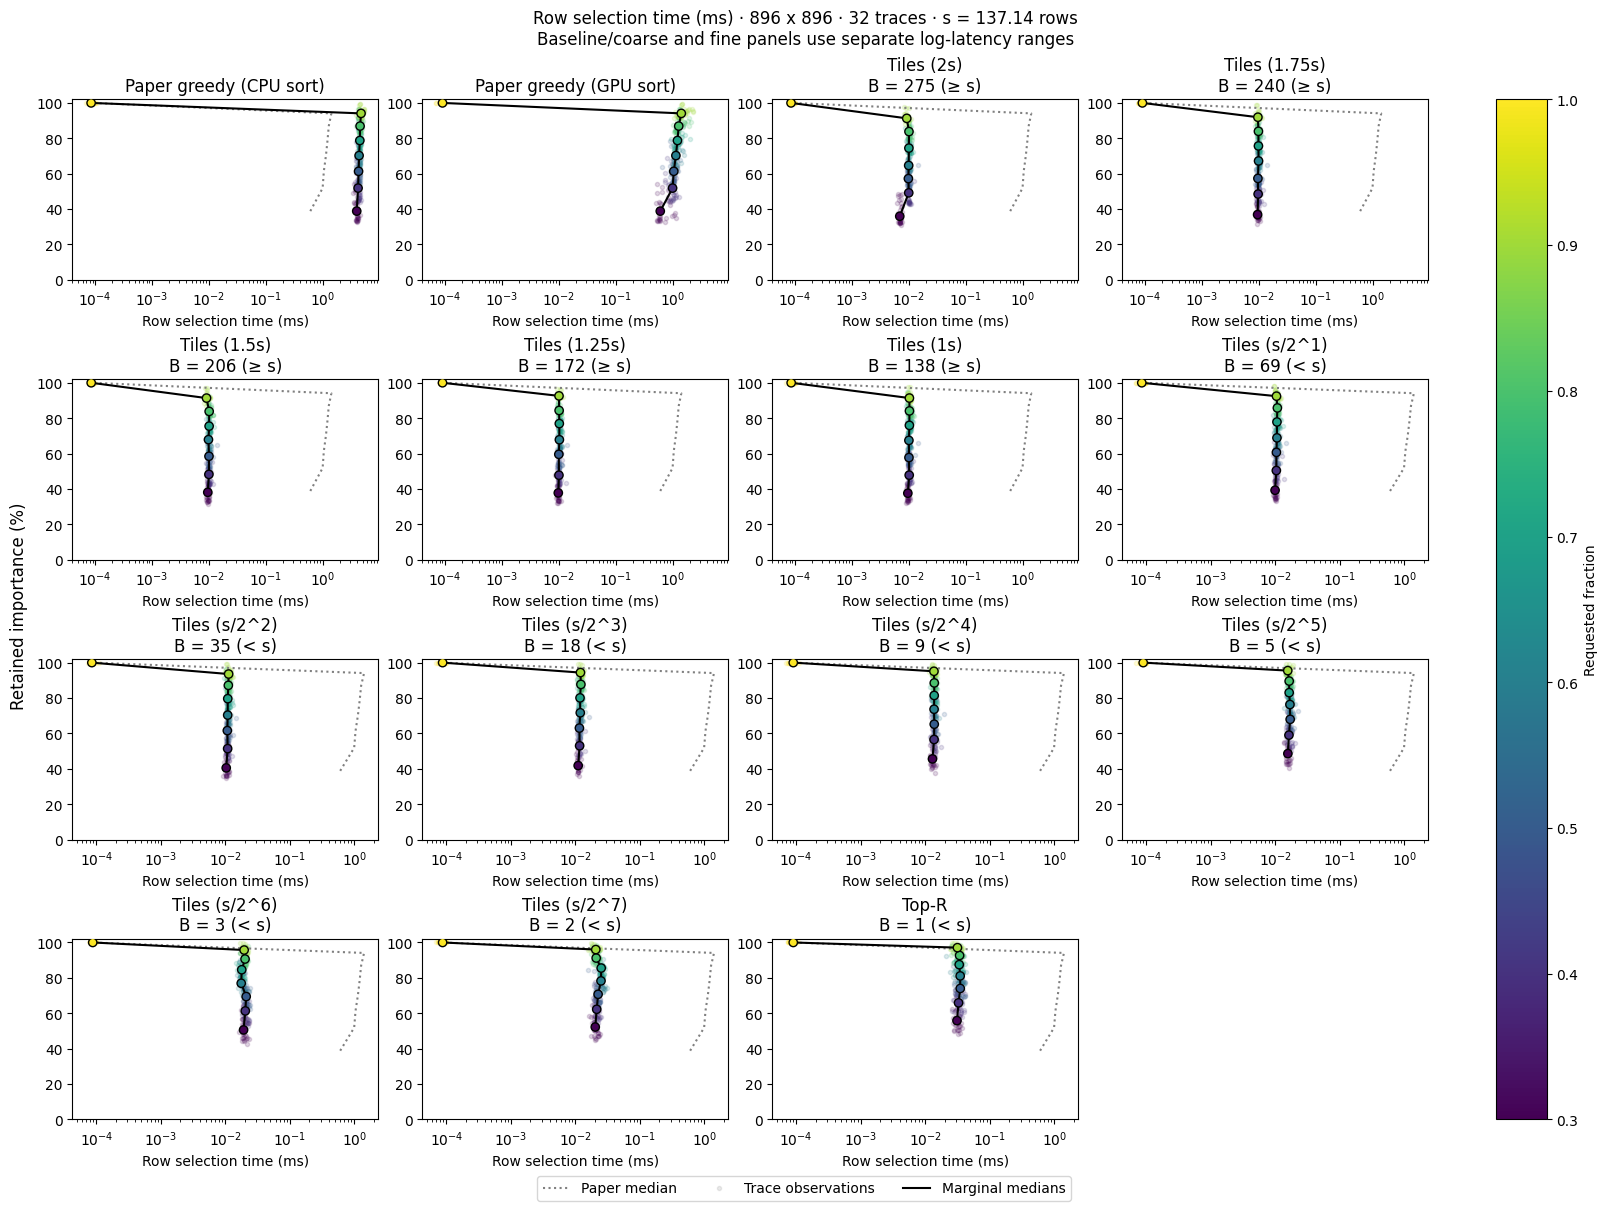
\includegraphics[width=0.85\textwidth]{figures/03/01_selection_latency_896x896.png}
    \caption{보존 중요도와 선택 시간. 색은 요청 비율을 나타내며, 그림의 s는 240 KiB를 행 단위로 환산한 기준이다. Baseline/coarse와 fine 패널은 서로 다른 가로축 범위를 사용하고, 가로축은 로그 척도이다.}
    \label{fig:real-selection}
\end{figure}

\textbf{읽기 시간}의 방법 간 관계는 \ref{sec:exp-model}절에서 비용 모델로 추정한 관계와 같았다. Tiles와 Paper의 읽기 시간은 0.4 ms 안팎으로 비슷하고, Top-$R$은 그 약 다섯 배이다. \ref{sec:exp-model}절의 추정에서는 이 차이가 열 배를 넘었으므로, 차이의 크기는 추정보다 작았다.

\begin{figure}[p]
    \centering
    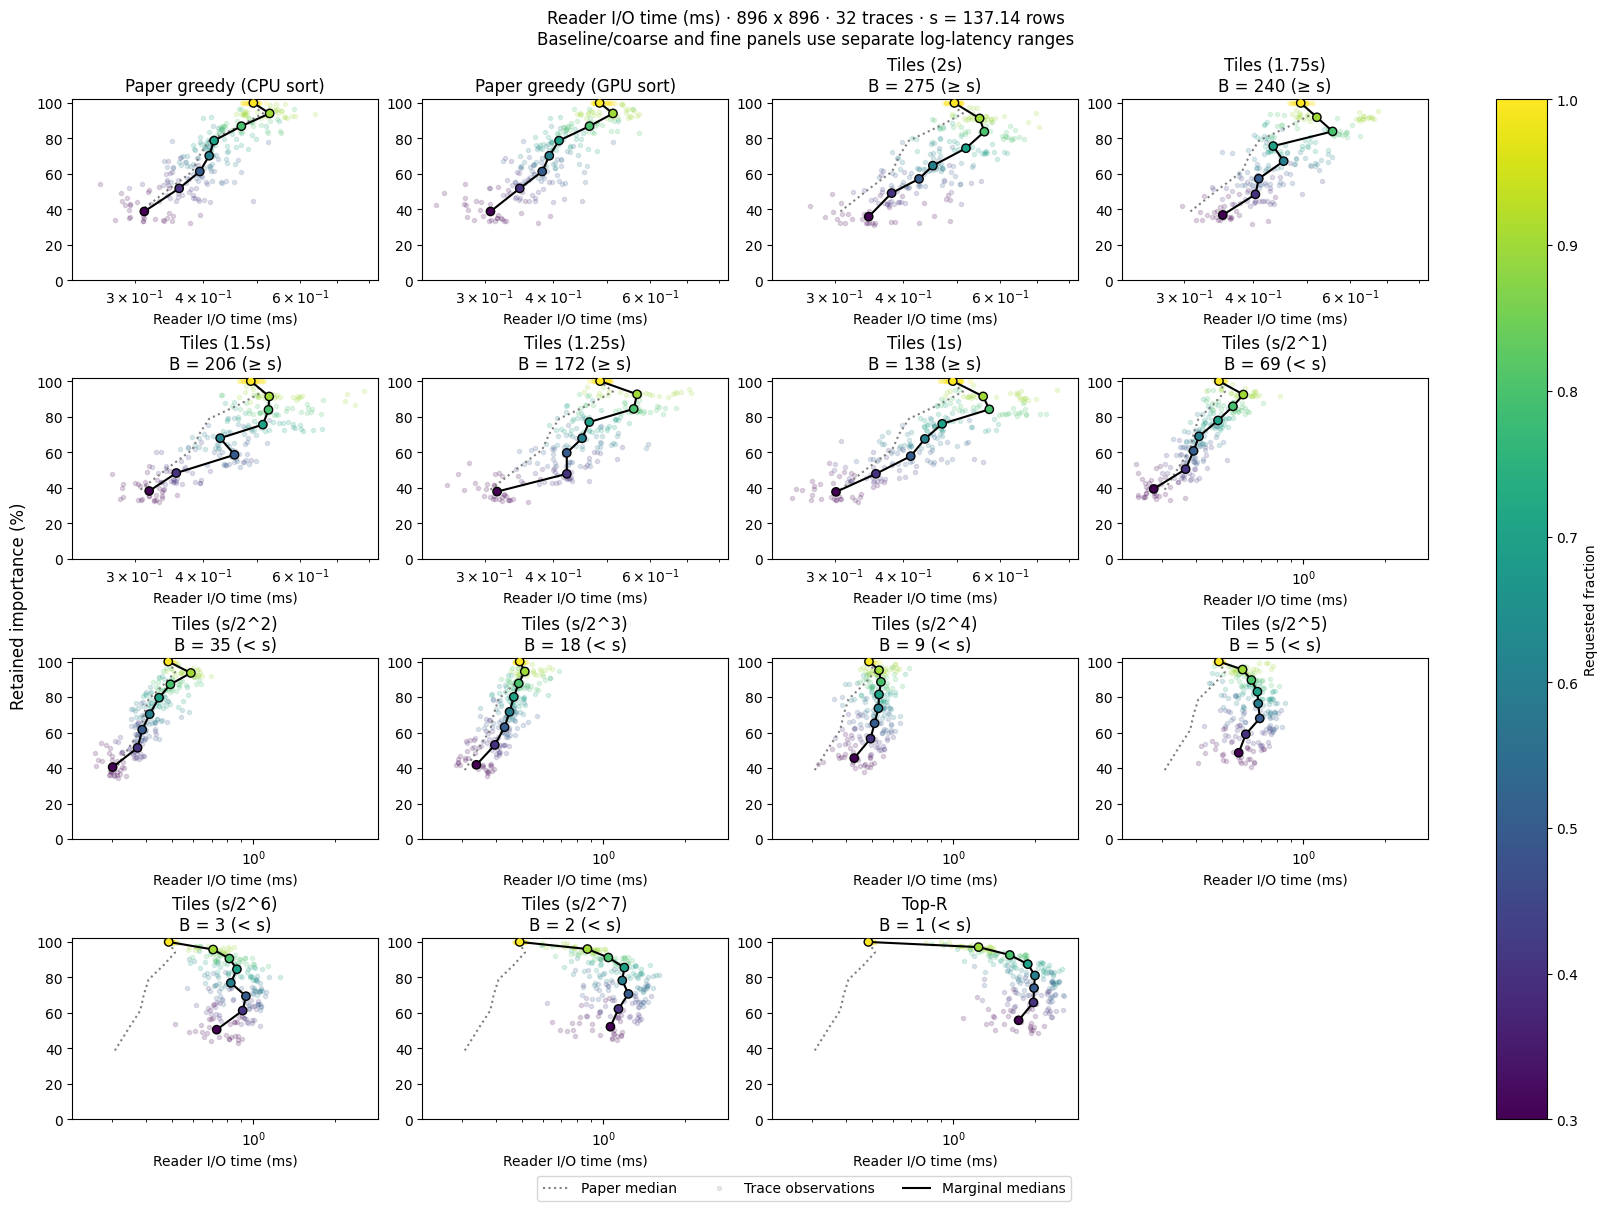
\includegraphics[width=0.85\textwidth]{figures/03/01_io_latency_896x896.png}
    \caption{보존 중요도와 읽기 시간.}
    \label{fig:real-io}
\end{figure}

\begin{figure}[p]
    \centering
    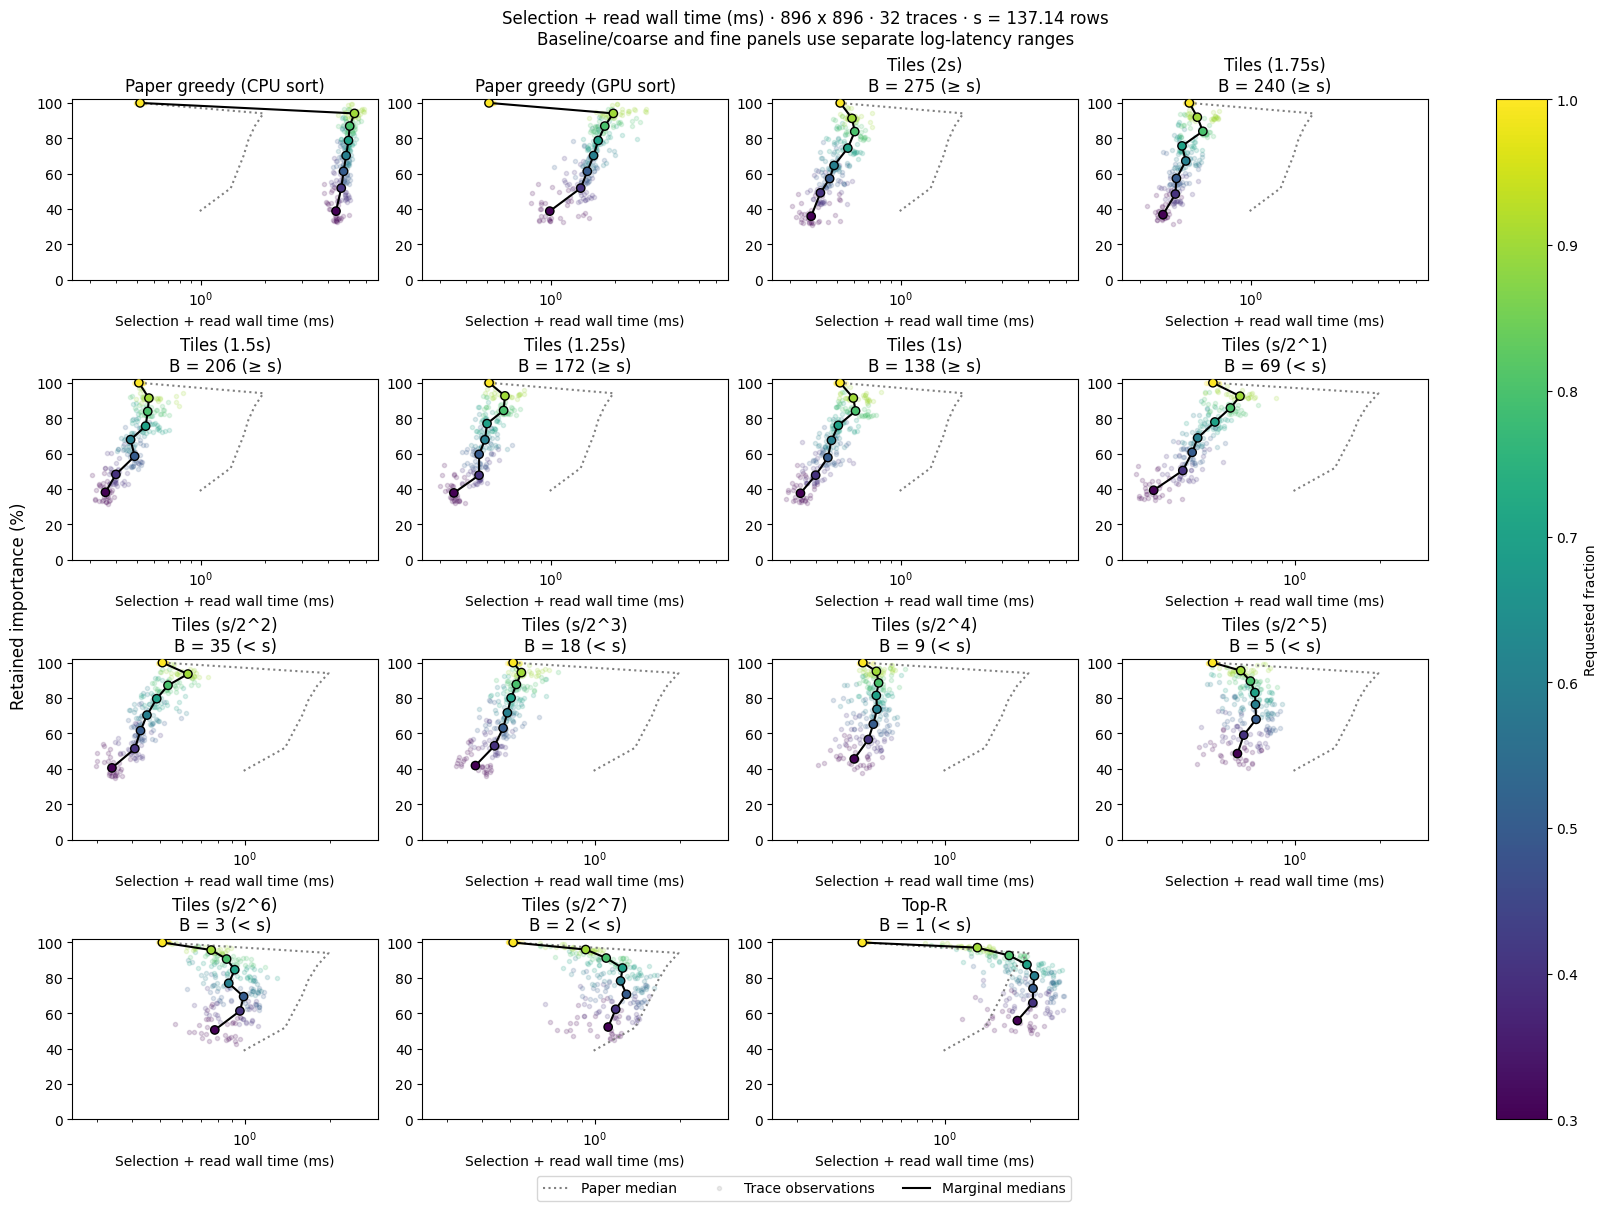
\includegraphics[width=0.85\textwidth]{figures/03/01_wall_latency_896x896.png}
    \caption{보존 중요도와 선택·읽기 전체 시간.}
    \label{fig:real-wall}
\end{figure}

\textbf{전체 시간}은 Tiles가 가장 짧았다. Paper는 읽기보다 선택에 더 긴 시간을 쓰므로, 읽기 시간이 비슷한데도 Tiles의 전체 시간은 Paper(GPU 정렬)의 약 3분의 1이다. Top-$R$은 선택은 빠르지만 읽기 시간이 길어, 전체 시간이 Tiles의 네 배를 넘었다. 한편 Tiles의 보존 중요도는 Paper보다 3.6\%p 낮았다.

나머지 shape에서도 같은 관계가 나타나는지 보기 위해, 같은 trace와 요청 예산끼리 짝지어 Tiles의 측정값에서 Paper의 측정값을 뺐다. Tiles는 각 shape의 기준 길이 $B=\lceil s\rceil$을, Paper는 GPU 정렬을 사용하였다. 표~\ref{tab:real-diff}\는 shape마다 32개 trace와 8개 예산의 256쌍에서 구한 차이의 중앙값이다. 시간의 차이가 음수이면 Tiles가 더 짧다는 뜻이다.

\begin{table}[htbp]
    \centering
    \caption{Shape별 Tiles에서 Paper(GPU 정렬)를 뺀 차이 (256쌍의 중앙값)}
    \label{tab:real-diff}
    \begin{tabular}{lrrrr}
        \toprule
        $N\times D$ & 보존 중요도 (\%p) & 선택 시간 (ms) & 읽기 시간 (ms) & 전체 시간 (ms) \\
        \midrule
        $896\times128$ & $+0.52$ & $-0.17$ & $+0.00$ & $-0.17$ \\
        $896\times896$ & $-1.82$ & $-1.07$ & $+0.02$ & $-1.05$ \\
        $896\times4864$ & $-1.11$ & $-1.11$ & $+0.06$ & $-1.03$ \\
        $4864\times896$ & $-0.83$ & $-1.93$ & $+0.11$ & $-1.86$ \\
        \bottomrule
    \end{tabular}
\end{table}

읽기 시간은 모든 shape에서 Tiles가 조금 길었으나, 그 차이는 가장 큰 $4864\times896$에서도 0.11 ms였다. 선택 시간의 차이가 이보다 훨씬 커서, 전체 시간은 모든 shape에서 Tiles가 짧았다. 보존 중요도는 $896\times128$을 제외한 세 shape에서 Tiles가 약 1--2\%p 낮았다.

% 작성 근거: 기존 노트북, 환경 기록, 저장된 CSV와 그림을 읽어 작성하였다. 측정 실험은 재실행하지 않았으며, 종류별 시간 그림과 차이 표는 저장된 CSV로 분석 노트북을 다시 실행하였다.
% Paper 튜닝: ../../results/03/03_01_tune_paper.ipynb
% 측정: ../../results/03/03_02_measure_latency.ipynb
% 실측 환경·튜닝 설정: ../../results/03/environment.json
% 그림 fig:real-selection: ../../results/03/03_03_compare_methods.ipynb, selection_ms-plot 셀의 두 번째 image/png 출력
% 그림 fig:real-io: ../../results/03/03_03_compare_methods.ipynb, io_ms-plot 셀의 두 번째 image/png 출력
% 그림 fig:real-wall: ../../results/03/03_03_compare_methods.ipynb, wall_ms-plot 셀의 두 번째 image/png 출력
% PNG는 각 노트북의 저장된 출력에서 그대로 추출하였다.
% 50% 예산 표의 수치: ../../results/03/03_05_report_numbers.ipynb (cases.csv, timings.csv에서 계산)
% 시간은 case_id별로 30회 반복의 중앙값을 구한 뒤 cases.csv에 결합하였다.
% 50% 예산 표는 n = d = 896, fraction = 0.5에서 방법별 32개 trace의 중앙값이다.
% Shape별 차이: ../../results/03/03_03_compare_methods.ipynb, 4. Paired differences 출력의 Tiles (1s) 행. trace_id와 fraction을 맞춰 Tiles (1s) - Paper greedy (GPU sort)를 계산한 뒤 각 shape의 256쌍에 대한 중앙값을 구하였다. 표에는 소수 둘째 자리까지 적었다.
% 중요도는 cases.csv의 retained_pct를 사용하였다.
% Reader의 시간 범위·분할·정렬 처리: ../../vlm-flash/src/vlmflash/csrc/native.cc
% Tiles 구현: ../../results/03/selectors.cpp
